% !TEX root = main.tex

\chapter[Complex Numbers and Functions]{Preliminaries on Complex Numbers and Functions}

\section{Basic Definitions and Algebraic Operations}

Formally, a \emph{complex number} is an ordered pair $(x,y)$ of real numbers.  We denote the set of all complex numbers by $\mathbb{C}$, and define addition and multiplication on $\C$ as follows:
\begin{enumerate}
\item[(i)] $(x_1,y_1)+(x_2,y_2) = (x_1+x_2,y_1+y_2)$,
\item[(ii)] $(x_1,y_1)(x_2,y_2) = (x_1x_2-y_1y_2,x_1y_2+x_2y_1)$.
\end{enumerate}
With this definition, $\C$ and $\R^2$ are equal \emph{as sets}, however, we have also defined an operation of multiplication on $\C$.


The subset of $\C$ given by 
\[
\set{(x,0): x \in \R } 
\]
is called the \emph{real axis}.  For complex numbers in this subset we have
\begin{align*}
(x_1,0)+(x_2,0) & = (x_1+x_2,0) \\
(x_1,0)(x_2,0) &= (x_1x_2,0), 
\end{align*}
so these complex numbers behave exactly like real numbers.  For this reason, we shall use $\R$ to refer to the real axis and denote the complex number $(x,0)$ by $x$.



Writing $i=(0,1)$, the definition of multiplication in $\C$ gives $i^2=-1$. With this notation, we get a more familiar `definition': a complex number $z=(x,y)$ can be written as
\begin{align*}
z = (x,y) &= (x,0)+(y,0)(0,1) \\
& = x + iy.
\end{align*}


The real numbers $x$ and $y$ are the \emph{real} and \emph{imaginary} parts of $z$ respectively, and we often write
\[
\Re (z) = x,\quad \Im (z)=y.
\]
Note that the imaginary part of $z$ is \emph{real}.   

With this more familiar notation, the algebraic operations of addition and multiplication on $\mathbb{C}$ can be expressed as follows: for $z_1=x_1+iy_1$ and $z_2=x_2+iy_2 \in \mathbb{C}$, we have
\begin{align*}
z_1 +z_2  &= (x_1+x_2) + i (y_1+y_2) \\
z_1z_2 & = (x_1+iy_1)(x_2+iy_2) \\
& = x_1x_2 + i (x_1y_2) + i (y_1x_2) + (i)^2(y_1y_2) \\
& = (x_1x_2-y_1y_2) + i (x_1y_2+x_2y_1).
\end{align*}


Note in particular that for $r \in \R$ and $z = x+iy \in \C$ we have
\[
rz = r(x+iy) = rx+iry.
\]





It is convenient to identify the complex number $z \in \C$ with the point (or sometimes, the vector) $(\Re (z), \Im (z) ) \in \R^2$.  Obviously the map $z \mapsto ( \Re (z), \Im (z))$ is a bijection $\C \to \R^2$, and thus geometrically, we view $\C$ as $\R^2$.




\begin{definition}[Complex Conjugate]
Given $ z \in \mathbb{C}$, the \emph{complex conjugate} $\overline{z}$ of $z$ is defined as
\[
\overline{z} := \Re (z) - i\ \Im (z). 
\]
\end{definition}

\begin{definition}[Modulus]
Given $z \in \mathbb{C}$, we define the modulus of $z$ to be
\[
| z | : = \sqrt{ \Re (z)^2 + \Im (z)^2 }.
\]
\end{definition}
\
In other words, for $z=x+iy$, $\conj{z}=x-iy$ and $\abs{z} = \sqrt{x^2+y^2}$.


Geometrically, the complex conjugate of $z$ describes the reflection of $z$ through the real axis, and the modulus of $z$ is the distance of $z$ from the origin.


\begin{proposition}
\label{p:absmod}
Let $z,z_1,z_2 \in \C$ be given.
Then:
\begin{enumerate}
%\item $i^2 = -1$.
\item[(i)] $\conj{\conj{z}} = z$ and $\abs{\conj{z}} = \abs{z}$.
\item[(ii)] $\abs{z} = \sqrt{\conj{z}z}$
\item[(iii)] $\conj{z_1+z_2} = \conj{z_1} + \conj{z_2}$ and $\conj{z_1z_2} = \conj{z_1}\ \conj{z_2}$.
\item[(iv)] $\conj{z} = z$ if and only if $z$ is real, i.e., if and only if $\Im (z)=0$.
\item[(v)] $\Re (z) = \displaystyle\frac{z + \conj{z}}{2}$ and $\Im (z) = \displaystyle\frac{z - \conj{z}}{2i}$.
\item[(vi)] $\abs{z} = 0$ if and only if $z = 0$.
\item[(vii)] $\abs{z_1 \pm z_2} \leq \abs{z_1} + \abs{z_2}$ \emph{(Triangle Inequality)}.
\item[(viii)] $\abs{z_1 \pm z_2} \geq \abs{\abs{z_1} - \abs{z_2}}$ \emph{(Reverse Triangle Inequality)}.
\item[(ix)] $\abs{z_1z_2} = \abs{z_1} \abs{z_2}$.
\end{enumerate}
\end{proposition}
You really should be familiar with all of these properties.  I would suggest trying to prove at least some of them, or verifying them for some specific choices of $z_1$ and $z_2$. Most of the proofs are short.

\begin{question}
The rules of multiplication allow us to divide a complex number $z$ by a nonzero real number $r$; i.e.
\[
\frac{z}{r} = \left( \frac{1}{r} \right) z.
\]
How do we define division of complex numbers?
\end{question}
\begin{answer}
For a complex number $z \neq 0$, we first define the multiplicative inverse of $z$, denoted $z^{-1}$ or $\frac{1}{z}$.  Note that  by Proposition~\ref{p:absmod} (ii), we have $\abs{z}^2 = z \conj{z}$.  Since $\abs{z}$ is real, we may  define the complex number
\[
\frac{\conj{z}}{\abs{z}^2}
\]
which must satisfy
\[
z \brac{ \frac{\conj{z}}{\abs{z}^2} } = \frac{z \conj{z}}{z \conj{z}} = \frac{\abs{z}^2}{\abs{z}^2} = 1.
\]
It follows that the multiplicative inverse of $z$ is
\[
z^{-1} = \frac{\conj{z}}{\abs{z}^2}.
\]
With this in mind, we may divide any complex number $z_1$ by any nonzero complex number $z_2$ as follows:
\[
\frac{z_1}{z_2} = z_1 z_2^{-1} = \frac{z_1\conj{z_2}}{\abs{z_2}^2}.
\]
\end{answer}

\begin{definition}[Argument]
The \emph{argument} of a complex number $z \neq 0$ is the angle $\arg (z)$ from the positive real axis to the vector representing $z$ in the anticlockwise direction.  
\end{definition}
Of course negative values of $arg(z)$ are allowed: these values represent angles taken in the clockwise direction.  Note that there are typically many ways in which we can represent $\arg (z)$, since we identify any two angles that differ by an integer multiple of $2\pi$ with one another.  For instance, for (the complex number) $z=1$ any of the angles
\[
\ldots,-4\pi, -2\pi, 0, 2 \pi , 4\pi,\ldots
\]
are valid choices for $\arg (z)$.   Similarly, if we look at $z=-1-i$:
%\begin{center}
%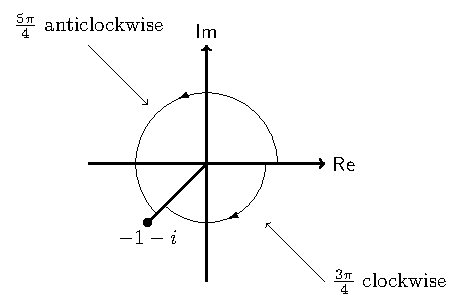
\includegraphics[scale=1]{arg}
%\end{center}
We can write $\arg (z) = \frac{5\pi}{4}$ or $\arg (z)=- \frac{3\pi}{4}$ (or indeed an integer multiple of $2\pi$ added to either of these angles).




By convention we usually take $\arg (z) \in (-\pi , \pi]$.
\begin{definition}
For $z \in \C$, $z \neq 0$, we define the \emph{Principal argument of $z$} (or the \emph{Principal value of $\arg(z)$}) to be the value of $\arg (z)$ that lies in $(-\pi,\pi]$. We shall denote this value by $\Arg (z)$.
\end{definition}
So for $z=-1-i$ we have $\Arg (z) = - \frac{3 \pi}{4}$, while $\arg (z)$ can be taken to be any of the values
\[
\ldots, - \frac{11\pi}{4}, - \frac{3\pi}{4}, \frac{5\pi}{4}, \frac{13\pi}{4}, \ldots.
\]


\begin{definition}
The \emph{polar form} of a complex number $z$ is given by writing $z$ in the form
\[
z = r \left( \cos (\theta) + i \sin (\theta) \right),
\]
where $r , \theta \in \R$ and $r \geq 0$.
\end{definition}
The polar form of $z$ is found by setting $r = \abs{z}$ and $\theta = \arg (z)$ (any value of $\arg(z)$ will of course suffice).  Equivalently, we may write
\[
z = r e^{i \theta}
\]
(though we have yet to define the complex exponential function).  For completeness, we should specify that the polar form of $0$ is simply $0$, since $\arg (0)$ is not defined.



\begin{definition}
Let $w=r \left( \cos( \theta) + i \sin ( \theta) \right)$ be (the polar form of) a complex number.  Then the $n^{th}$ \emph{complex roots} of $w$ are defined to be the $n$ solutions $z_0, z_1, \ldots , z_{n-1}$ of the equation $z^n = w$.  These roots are given by
\[
z_k = \sqrt[n]{r} \left( \cos \left( \frac{\theta+2k \pi}{n} \right) + i \sin \left( \frac{\theta + 2k\pi}{n} \right) \right),
\]
for $k=0,1,\ldots,n-1$, where $\sqrt[n]{r}$ is the (positive) $n^{th}$ real root of $r$.
\end{definition}


\begin{figure}[H]
\centering
\begin{tabular}{cc}
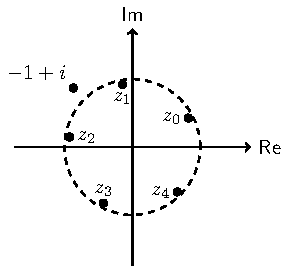
\includegraphics{ch1_sqrt1} & 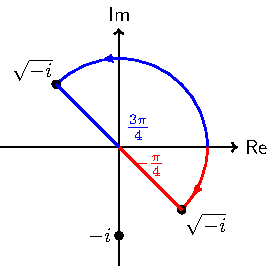
\includegraphics[scale=1]{ch1_sqrt2}
\end{tabular}
\caption{The 5\textsuperscript{th} roots of $z=-1+i$ (left), and the two square roots of $-i$ (right).}.
\end{figure}


\begin{theorem}
Let $z_1$ and $z_2$ be nonzero complex numbers.  Then
\begin{enumerate}
\item[(i)] $\abs{z_1z_2}=\abs{z_1} \ \abs{z_2}$, and
\item[(i)] $\arg (z_1z_2)=\arg(z_1)+\arg(z_2)$.
\end{enumerate}
\end{theorem}
{\bf Proof:} Exercise.


\section{Complex Functions}

We now start our investigation of functions from the complex plane to itself.  First of all, note that a function $\mathbf{f}:\R^2 \to \R^2$ can be written in the form
\[
\mathbf{f}(x,y)=\left( u(x,y), v (x,y) \right)
\]
where $u,v:\R^2 \to \R$.  For example, if
\[
\mathbf{f}(x,y)=\left(x^2+y^2-2x,2y-6 \right),
\]
we have
\[
u(x,y)=x^2+y^2-2x \text{ and } v(x,y)= 2y-6.
\]





Since we have a formal definition of $\C$ as $\R^2$, we can express a function $f : \C \to \C$ as
\begin{equation*}
f(z) = f(x+iy) = u(x,y) +i v(x,y)
\end{equation*}
for all $z =x+iy \in \C$, where $u, v : \R^2 \to \R$.  In this way, we can extend our definition of real and imaginary parts from complex numbers to functions $f:\C \to \C$, writing $\Re (f) = u$ and $\Im (f) = v$.




Going in the other direction, given two functions $u:\R^2 \to \R$ and $v:\R^2 \to \R$, we can create a function $f : \C \to \C$ by \emph{defining} $f(x+iy) := u(x,y) +iv(x,y)$.
So,
\begin{center}
\emph{
 There is a correspondence between functions from the complex plane to itself, and pairs of functions from the real plane to the real line.}
 \end{center}




\begin{example}
The function \[ f: \C \to \C,\quad f(z) = \conj{z} \]
corresponds to a function
\[ \mathbf{f}: \R^2 \to \R^2, \quad \mathbf{f}(x,y) = \left( u(x,y), v(x,y) \right)
\]
\begin{blankbox}
\[
u(x,y) = x\ \qquad\text{and}\qquad v(x,y) = -y
\]
since
\[
\conj{z} = \conj{x+iy} = x-iy = \underbrace{x}_{u(x,y)} + i \underbrace{(-y)}_{v(x,y)}.
\]
\end{blankbox}
\end{example}



\begin{example}

Let us determine the functions $u:\R^2 \to \R$ and $v:\R^2 \to \R$ corresponding to
\begin{equation*}
h: \C \to \C, z \mapsto z^2.
\end{equation*}
\end{example}
\begin{solution}
With $z=x+iy$ we have
\[
z^2 = (x+iy)^2 = x^2-y^2+i2xy
\]
Thus we identify $h:\C \to \C$ with $\mathbf{h}:\R^2 \to \R^2$, $\mathbf{h}(x,y) = (u(x,y), v(x,y))$  where
\begin{gather*}
u: \R^2 \to \R, \quad u(x,y) = x^2-y^2, \\
v: \R^2 \to \R, \quad v(x,y) = 2xy.
\end{gather*}

\end{solution}

\begin{comment}
\begin{example} Let us find the corresponding complex function, $f:{\mathbb C} \rightarrow {\mathbb C}$, for the function
\begin{equation*}
\mathbf{f} : \R^2 \to \R^2, (x,y) \mapsto (2y,-x)
\end{equation*}
and express it in terms of $z \in \C$.
\end{example}

%\begin{master}
\begin{solution}
The corresponding function $f:\C \to \C$ is given by
\begin{align*}
f(z)= f(x+iy)&=2y+i(-x) \\
& = 2 \Im (z) +i ( - \Re (z) ) \\
& = 2 \left( \frac{z-\overline{z}}{2i} \right)-i \left( \frac{z+\overline{z}}{2} \right) \\
&=\frac{-3i z}{2}+\frac{i\overline{z}}{2}.
\end{align*}

Thus the corresponding complex function is
\begin{equation*}
f: \C \to \C, \ f(z)= \frac{-3i z}{2}+\frac{i\overline{z}}{2}.
\end{equation*}
(Here we have used the identities $\Re (z) = \frac{1}{2} (z+\conj{z})$ and $\Im (z) = \frac{1}{2i}(z-\conj{z})$, together with the fact that $i^{-1}=-i$)
\end{solution}
%\end{master}
%\vspace*{5cm}
\end{comment}




\begin{example}
Let find the complex function $f$ corresponding to the function $\mathbf{f}:\R^2 \to \R^2$ where
\begin{enumerate}
\item[(i)] $\mathbf{f} (x,y) = (-2y+3,2x),$ and
\item[(ii)] $\mathbf{f}(x,y) = (x^2+y^2-2x,2y-6)$.
\end{enumerate}

\end{example}

\begin{solution}
We could use the fact that if $z=x+iy$ then
\begin{align*}
x & = \Re(z) = \frac{1}{2} \left( z+ \conj{z} \right) \\
y & = \Im (z) = \frac{1}{2i} \left( z- \conj{z} \right).
\end{align*}
Substituting these expressions for $x$ and $y$, we could then simplify and find $f(z)$. However, this is time consuming, and it is sometimes easier to look for familiar expressions in the definition of $f$.

In part (i), $\mathbf{f}$ corresponds to $f: \C \to \C$ defined by
\begin{align*}
f(z) = f(x+iy) &= -2y+3+i(2x) \\
& = 2(ix-y) + 3 \\
& = 2(ix+i^2y)+3 \\
& = 2i(x+iy)+3 \\
& = 2iz+3.
\end{align*}

In part (ii), $\mathbf{f}$ corresponds to $f:\C \to \C$ where
\[
f(x+iy) = x^2+y^2-2x+i2y-6i.
\]
With $z=x+iy$, notice that
\[
x^2+y^2=\abs{z}^2 = z \conj{z},
\]
and that
\[
-2x+i2y = -2 (x-iy) = -2 \conj{z},
\]
hence
\[
x^2+y^2-2x+i2y-6i = z \conj{z} - 2 \conj{z} -6i.
\]
Hence $f(z) = z \conj{z}-2\conj{z}-6i$ is the corresponding complex function.



\end{solution}




It is worth recalling that some familiar functions defined on $\R$ extend to $\C$.

\begin{definition}
\label{d:exp}
The \emph{exponential function} is the function $\exp : \C \to \C$ defined by
\[
\exp (x+iy) = \exp(x) \left( \cos (y) + i \sin (y) \right)
\]
for all complex numbers $x+iy \in \C$, where $\exp (x) (=e^x)$ is the usual (real) exponential of $x$.
\end{definition}
We shall often write $e^z$ in place of $\exp (z)$.   The trigonometric functions also extend to $\C$ via
\begin{align}
\cos (z) &= \frac{1}{2} \left( \exp (iz) + \exp (-iz) \right) \\
\sin (z) & = \frac{1}{2i} \left( \exp(iz)- \exp (-iz) \right).
\end{align}




\begin{full}
\begin{remark}
We conclude this section with some remarks about how you might go about `visualising' a complex function.  For functions $f:\R \to \R$, we usually do so by drawing the graph of $f$, that is, the subset $\set{(x,f(x)): x \in \R}$ of $\R^2$.

We cannot draw the `graph' of a function $f:\C \to \C$, as to do so would require four coordinates
\[
\set{ \Re (z), \Im (z) , \Re \left( f(z) \right), \Im \left( f(z) \right) }
\]
and thus four dimensions.  We can however view $f$ as a `transformation' of the complex plane, and examine the effect of applying $f$ to
\begin{itemize}
\item Regions (subsets) of $\C$
\item Curves in $\C$ (lines, circles etc)
\item A combination of the two.
\end{itemize}


\begin{figure}[H]
\centering
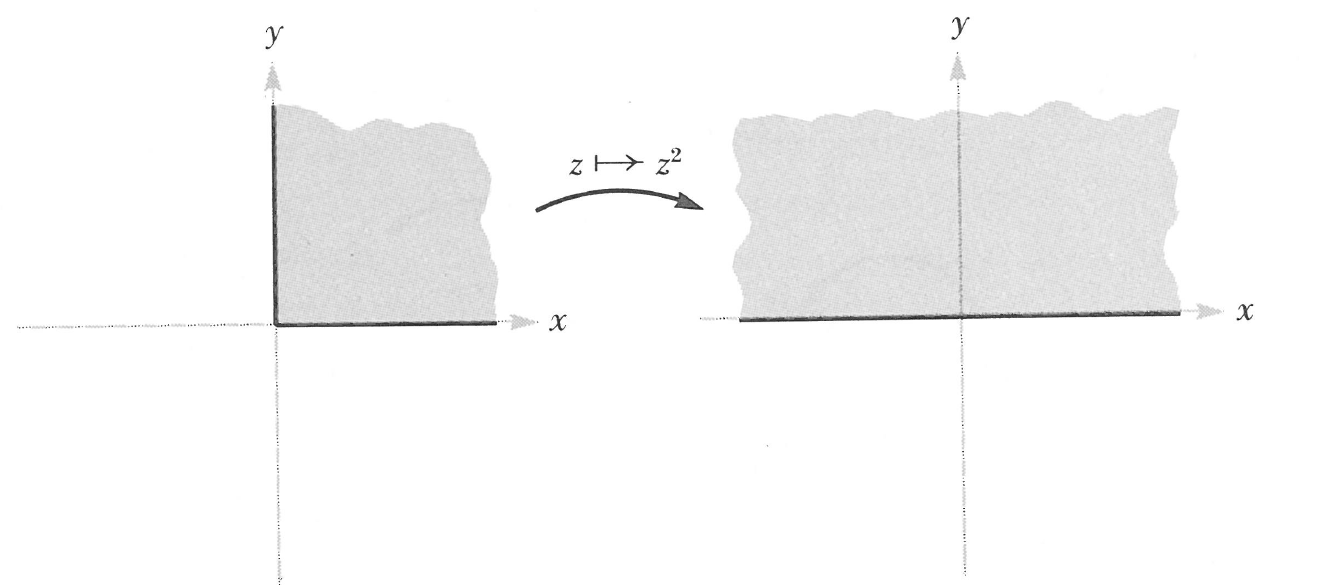
\includegraphics[scale=0.25]{ch1_z2quad}
\caption{The image of the first quadrant under $z \mapsto z^2$.}
\label{f:z2}
\end{figure}
Figure~\ref{f:z2} indicates that the image of the first quadrant under the map $z \mapsto z^2$ is the region consisting of the first and second quadrants.  This follows from the fact that for any $z_1,z_2 \in \C$, 
\[
\arg (z_1z_2)=\arg(z_1)+\arg(z_2).
\]
Hence $\arg(z^2)=2\arg(z)$, and so if $0 \leq \arg (z) \leq \pi/2$ (i.e. $z$ is in the first quadrant), we have $0 \leq \arg (z^2) \leq \pi$ ($z^2$ lies in either the first or second quadrant).  Of course, Figure~\ref{f:z2} does not tell us anything about the modulus of $z^2$.


Figure~\ref{f:z2c} illustrates how $z \mapsto z^2$ also squares the modulus; the circle of radius $r>0$ and centre $0$ is sent to the circle of radius $r^2$ and centre $0$.  Moreover, the anticlockwise arrows on the circles indicate that if $z_2$ lies (a small distance) anticlockwise of $z_1$, then $z_2^2$ lies anticlockwise of $z_1^2$.




%\vspace*{2cm}

\begin{figure}[H]
\centering
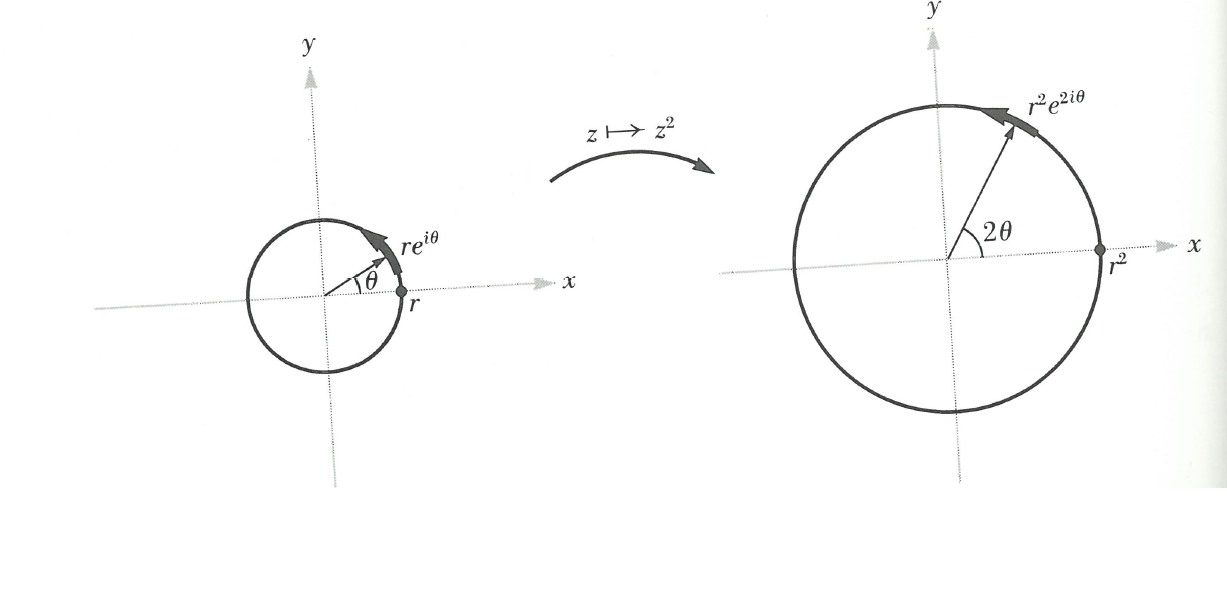
\includegraphics[scale=0.3]{ch1_z2circle}
\caption{The effect of the map $z \mapsto z^2$ on a circle of radius $r$ centred at the origin.}
\label{f:z2c}
\end{figure}

%\vspace{2cm}

\begin{figure}[H]
\centering
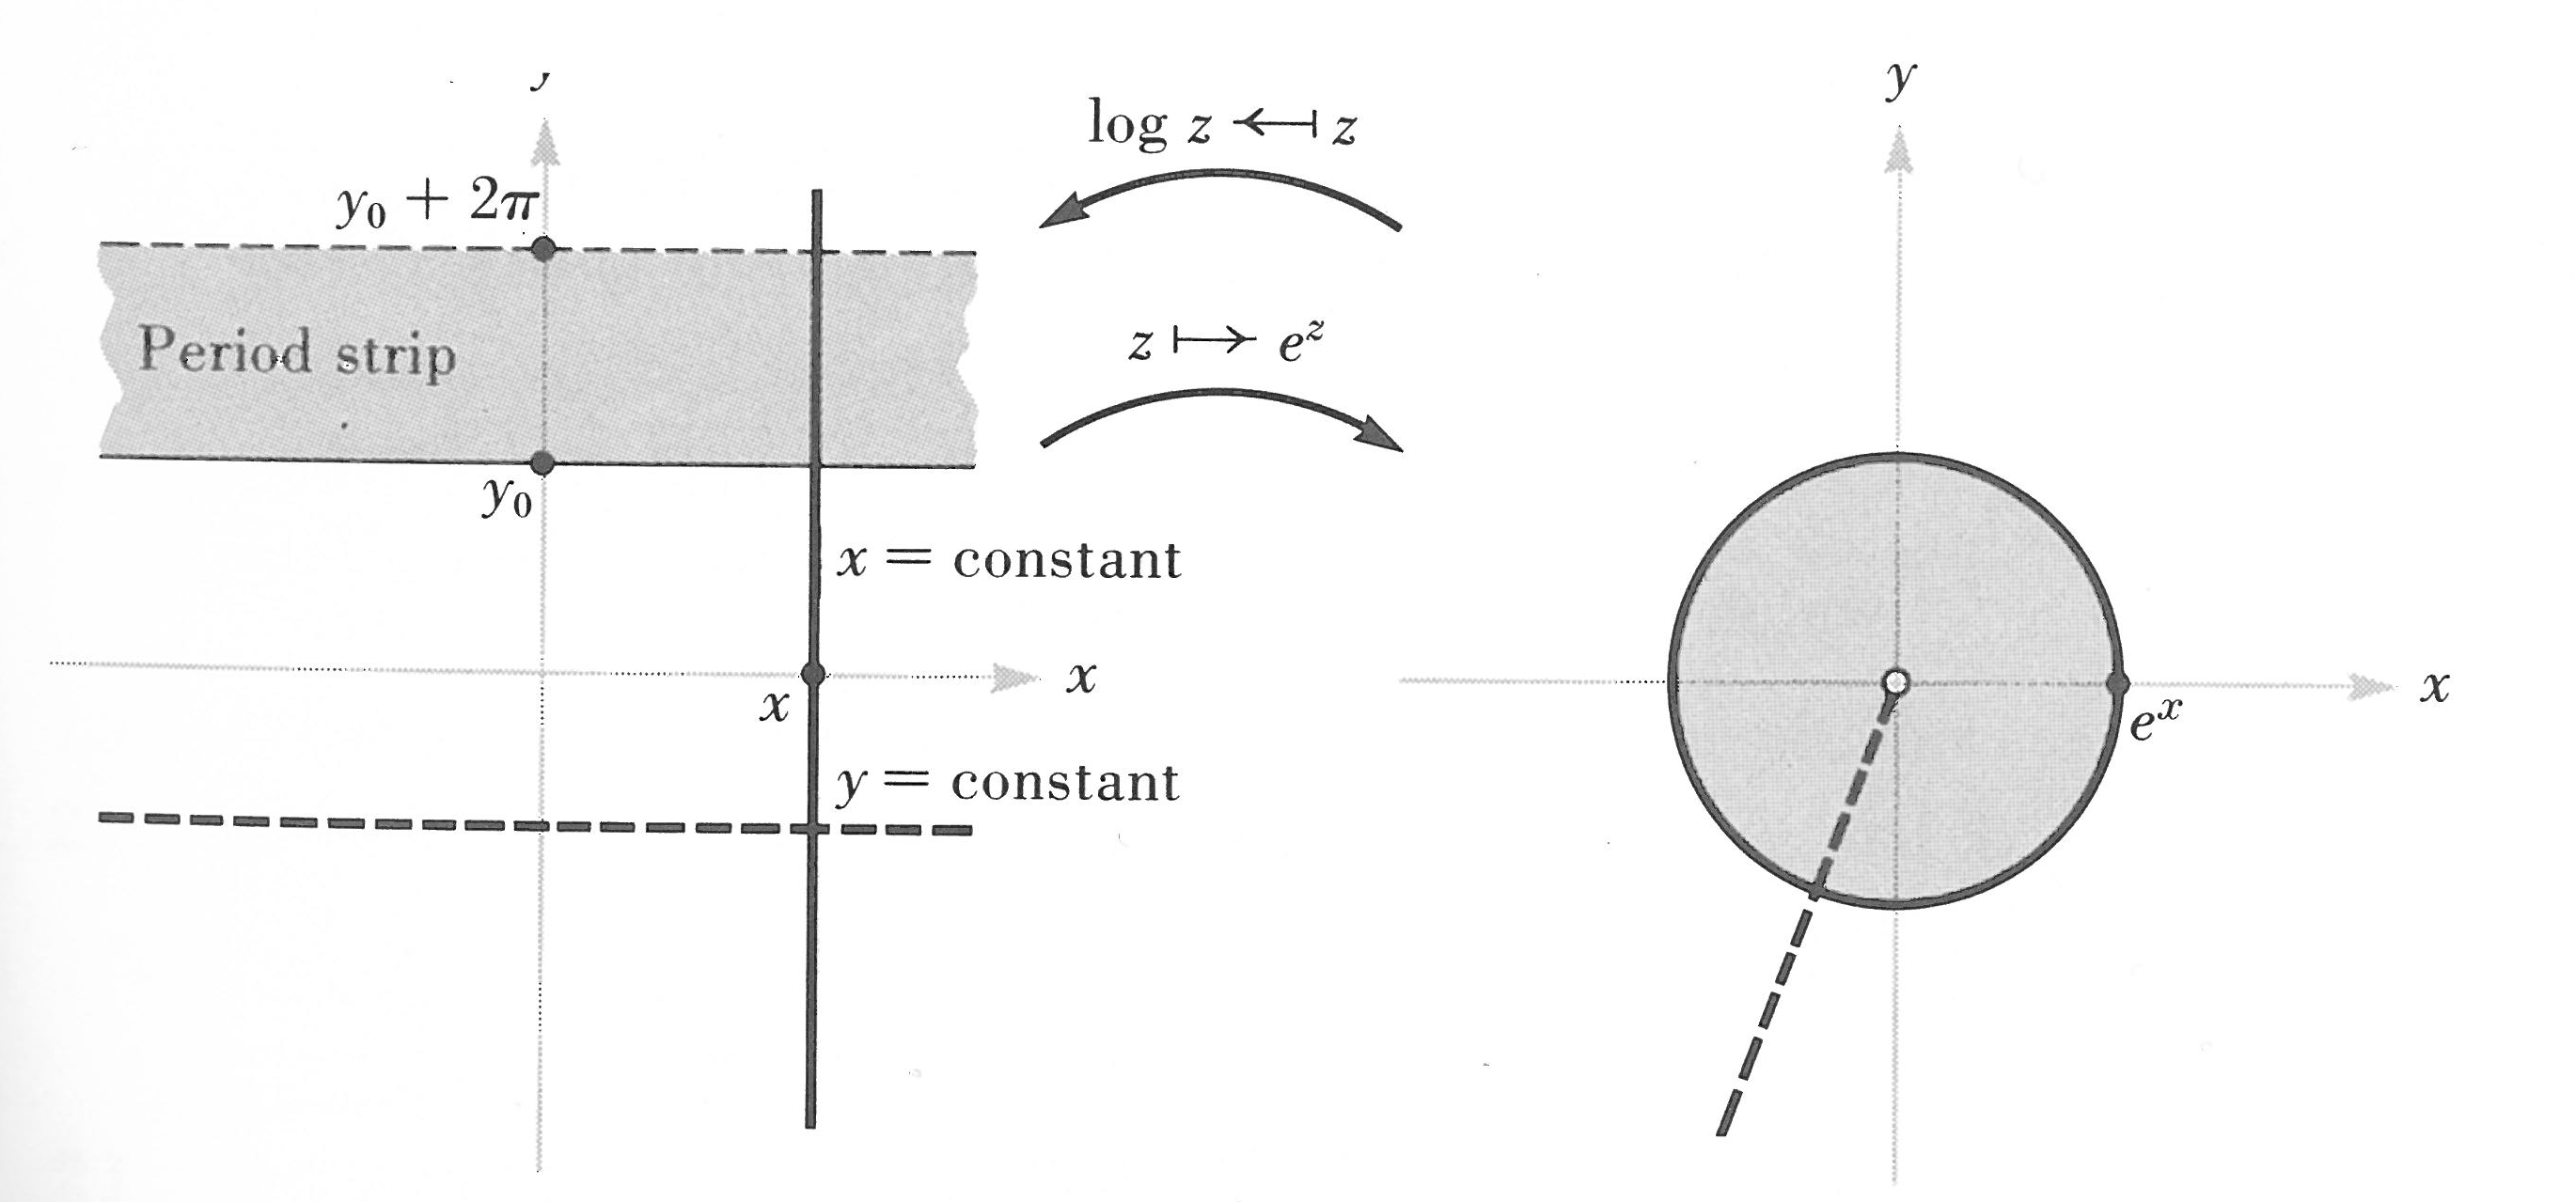
\includegraphics[scale=0.15]{ch1_expimage}
\caption{The geometric effect of the exponential map.}
\label{f:exp}
\end{figure}

Figure~\ref{f:exp} combines the approaches of the previous examples.  Here we see that the shaded region,
\[
\set{z \in \C: \Re (z) \leq x \text{ and } y_0 \leq \Im (z) < y_0+2\pi}
\]
is sent to the shaded disc of radius $e^x$ and centre $0$.  The vertical line $\Re(z)=x$ is sent to the circle of radius $e^x$ and centre $0$, while the dashed horizontal line is sent to the `infinite ray' from $0$ indicated with another dashed line.

Strictly speaking this diagram is inaccurate, as some of the region to the right of the line $\Re(z)=x$ is also shaded.

I will not ask you to produce diagrams like this in the exam, but it may be helpful to have the idea of complex functions as transformations in your mind throughout this module.
%\vspace{2cm}

%\vspace*{2cm}
Figures~\ref{f:z2},~\ref{f:z2c} and~\ref{f:exp} are from \emph{Basic Complex Analysis}, (Jerrold. E. Marsden, published by W.H. Freeman and Company, 1973).  

\end{remark}
\end{full}


\section{Open Sets in $\C$}




\begin{definition}[Open Disc]
Let $z_0 \in \C$ and let $r>0$ be some real number.  The open disc of radius $r$ centred at $z_0$ is defined to be the set 
\[
D(z_0,r):= \set{ z \in \C: \abs{z-z_0} <r}.
\]
\end{definition}
In other words, $D(z_0,r)$ is the set of all points that lie (strictly) inside the circle or radius $r$ with centre $z_0$.
\begin{definition}
The set of points
\[
D'(z_0,r) = \set{ z \in \C: 0 < \abs{z-z_0} < r},
\]
where $r>0$ and $z_0 \in \C$, is called the \emph{punctured open disc} of radius $r$, centre $z_0$.
\end{definition}



Note that $D'(z_0,r)$ is the set obtained by removing the centre $z_0$ from the open disc $D(z_0,r)$.
\begin{sfig}
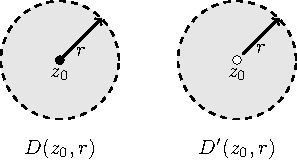
\includegraphics[scale=1]{ch1_discs}
\caption{The open disc $D(z_0,r)$ and punctured open disc $D'(z_0,r)$.}
\label{f:discs}
\end{sfig}

\begin{notation}
This is a good place to introduce some conventions for sketching sets.  The broken circle in Figure~\ref{f:discs} around the disc indicates that the boundary is not included in this set.  The filled point $\bullet$ beside $z_0$ indicates that the point $z_0$ is included in $D(z_0,r)$, while the `hollow' point $\circ$ beside $z_0$ indicates that $z_0$ is not included in the punctured disc $D'(z_0,r)$.
\end{notation}


\begin{definition}
Let $U \subseteq \C$, then we say that $U$ is an \emph{open set} if given any $z \in U$ there is some $r_z>0$ with $D(z,r_{z}) \subseteq U$.
\end{definition}
\begin{sfig}
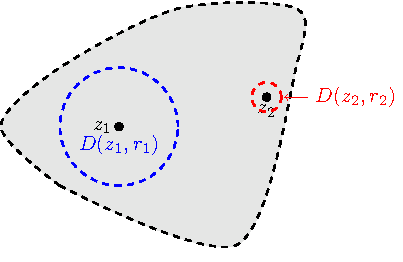
\includegraphics[scale=1]{ch1_openset}
\caption{An open set $U$ with two examples of open discs around points of $U$.  Note that the radius typically depends on the point $z$; points nearer the `edge' of $U$ will need smaller discs.}
\end{sfig}
Informally, we think of an open set as a set that does not include its `boundary.'  Thus a set $U$ is open if, given any $z \in U$, we can move a small distance in \emph{any} direction without leaving $U$.


\begin{example}
\begin{itemize}
\item[(i)] The open disc $D(0,1)$ is an open set.

\altgraphics[scale=1]{ch1_unit_disc_full}{ch1_unit_disc}

\begin{full}
Let $z \in D(0,1)$.  Our goal is to find some $r>0$ so that $D(z,r) \subseteq D(0,1)$. To this end, set $r= (1-\abs{z})/2$. Then if $w \in D(z,r)$,
\begin{align*}
\abs{w-0} & \leq \abs{w-z} + \abs{z} \\
& < \frac{1-\abs{z}}{2} +\abs{z} \\
&= \frac{1+\abs{z}}{2} < \frac{1+1}{2} = 1,
\end{align*}
which shows that $w \in D(0,1)$.

%\vspace*{2cm}
Hence $D(z,r) \subseteq D(0,1)$ and so $D(0,1)$ is open.
\end{full}

\item[(ii)] The closed disc $\overline{D} (0,1) := \set{ z \in \C: \abs{z} \leq 1 }$ is not an open set (note: \emph{closed} does not necessarily mean not open).
\leftimage{
\altgraphics[scale=1]{ch1_cldisc1}{ch1_cldisc1_full}
}
{
The solid circle in this image indicated that the boundary is included.
}


\begin{blankbox}
Given any point $z$ on the boundary (e.g. $z=1$) and any $r>0$, the open disc $D(z,r)$ contains points that do not belong to $\overline{D}(0,1)$. 
\end{blankbox}
\begin{full}
 For example, $w=1+r/2$ belongs to $D(1,r)$, since
\[
\abs{w-z} = \abs{(1+r/2)-1} = r/2 < r
\]
but not to $\overline{D} (0,1)$, since
\[
\abs{w-0} = \abs{1+r/2} = 1+r/2 >1.
\]
\end{full}

\end{itemize}
\end{example}



\begin{example}
 The upper-half plane $H_+$, where
\[
H_+ := \set{ z \in \C: \Im (z) > 0 }
\]
is an open set, while the set $K_+$ defined by
\[
K_+:= \set{ z \in \C : \Im (z) \geq 0 }
\]
is not.
\begin{center}
\altgraphics[scale=1]{ch1_upperhalf_full}{ch1_upperhalf} \quad \altgraphics[scale=1]{ch1_upperhalf2_full}{ch1_upperhalf2}
\end{center}
\begin{blankbox}
If $z \in H_+$ then $\Im (z)>0$, so we set $r = \frac{1}{2} \Im (z)$.  Then $D(z,r)\subseteq H_+$, or in other words, given any $w \in D(z,r)$, we must have $\Im(w)>0$.

For the set $K_+$, if we choose $z$ on the real axis (e.g $z=-1$), then any open disc centred at $z$, no matter how small, contains points below the real axis.  Thus there is no $r>0$ with $D(z,r) \subset K_+$, so $K_+$ is not open.
\end{blankbox}
\end{example}




\begin{note}
Some more examples of open sets include $\C \backslash \set{0}$, or indeed $\C \backslash F$ where $F$ is any finite set.  Many regions determined by \emph{strict} inequalities of real numbers are also open, for example, sets of the form
$
\set{ z \in \C: c_1<\abs{z}<c_2 }$, $\set{ z \in \C: 0 < \Arg (z) < \pi/4 }$ or $\set{z \in \C: c_1<\Re(z) < c_2 },$
where $c_1<c_2 $ are real numbers.

More examples of sets that are not open include circles, lines, curves, single points or finite sets.  Do not use \emph{closed} to mean \emph{not open}.  In the context of analysis, closed has a different meaning.
\end{note}
Throughout this module, we shall be mostly concerned with functions $f:U \to \C$, where $U$ is an open subset of $\C$.  

 
\section{Limits}
Limits in $\C$ are defined in an analogous way to those in $\R$ (and almost identically to those in $\R^2$). 

First, fix some complex number $z_0 \in \C$.  For any $z \in \C$, the modulus $\abs{z-z_0}$ measures the distance between $z$ and $z_0$.  Note that if we write $z=x+iy$ and $z_0=x_0+iy_0$, then $\abs{z-z_0}$ is exactly the same as the Euclidean distance between $(x,y)$ and $(x_0,y_0)$ in $\R^2$.




 For a complex function $f$, what does it mean to say that $f(z)$ approaches $L \in \C$ as $z$ approaches $z_0$?  \ Intuitively, we want
 \begin{center}
 $\abs{f(z)-L}$ is small whenever  $\abs{z-z_0}$ is small.
 \end{center}
  More formally, this can be written as
 \begin{center}
 Given any $\epsilon>0$ there is a $\delta>0$ such that
 \[
 \abs{f(z)-L} < \epsilon\text{ whenever } \abs{z-z_0}<\delta.
 \]
 \end{center}
 
 This definition works whenever $f$ is defined on all of $\C$, but it is not so clear how it should work when $f(z)$ is not defined near $z_0$. In other words, we want to be able to exclude points $z_0$ where $\abs{z-z_0}$ small implies $f(z)$ does not exist. 
 \begin{comment}
 Recall the following definition from Foundations II: given a set $A \subseteq \R$, a point $x_0$ is a \emph{limit point} of $A$ if whenever $I$ is an open interval with $x_0 \in I$, then $I$ contains an element of $A \backslash \set{x_0}$.
 
 We define limit points of subsets of $\C$ in almost exactly the same way, replacing open intervals with open discs.
 \end{comment}
 
 \begin{definition}
 A point $z_0$ is a \emph{limit point} of of a set $S \subseteq \C$  if for any $\delta>0$, we have
 \[
 D'(z_0,\delta) \cap S \neq \emptyset.
 \]
 In other words, any punctured disc centred at $z_0$, no matter how small, contains at least one point of $S$.
 \end{definition}

A limit point of a set $S$ may or may not belong to $S$.  Moreover, a point $z_0 \in S$ may or may not be a limit point of $S$.  If $S$ is an open set however, then any $z_0 \in S$ is necessarily a limit point of $S$.



\begin{example}
\begin{enumerate}
\item[(i)] The point $0$ is a limit point of the punctured plane $\C \backslash \set{0} = \set{ z \in \C : z \neq 0 }$.
\begin{center}
\altgraphics[scale=1]{ch1_pplane_full}{ch1_pplane}
\end{center}
\begin{blankbox}
Indeed, it is clear that every punctured disc $D'(0,r)$ contains points of $\C \backslash \set{0}$.  
\end{blankbox}

In fact, every point $z$ of $\C$ is a limit point of $\C \backslash \set{0}$, since every disc $D'(z,r)$ must contain a point of $\C \backslash \set{0}$.


\item[(ii)] If $S= \set{z_0}$ is a one-point set, then there are no limit points of $S$.  %Indeed, for any $\delta>0$, $D'(z_0,\delta)$ does not contain any points of $S$ by definition.  Moreover, given any other point $z\in \C$ with $z \neq z_0$, the punctured disc $D'(z,\delta)$, with $\delta = \frac{1}{2} \abs{z-z_0}$, does not contain $z_0$.

\item[(iii)] The set of limit points of the open disc $S=D(z_0,r)$ is precisely the closed disc
\[
\set{z \in \C: \abs{z-z_0} \leq r }.
\]
\begin{center}
\altgraphics[scale=1]{ch1_limitpoints_disc_full}{ch1_limitpoints_disc} 
%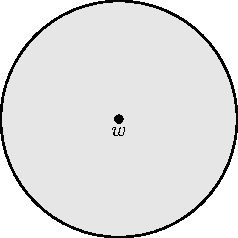
\includegraphics[scale=1]{cldisc_big}
\end{center}
\begin{blankbox}
For a point $z_1$ on the boundary, any punctured disc $D'(z_1,r)$ intersects $S$, while for a point $z_2$ outside of the boundary, there are punctured discs $D'(z_2,r_2)$ that do not.
\end{blankbox}

\item[(iv)] Let $L$ be the strictly positive real axis, regarded as a subset of $\C$, that is
\[
L = \set{ x+ iy \in \C: x>0 \text{ and } y=0 }.
\]
Then $z=0$ is a limit point of $L$.
\begin{center}
\altgraphics[scale=1]{ch1_halfline_full}{ch1_halfline}
\end{center}


%If $z_1$ is a point on the boundary of $D(w,r)$, then for any $\delta>0$, $D'(z_1,\delta)$ contains points of $D(w,r)$.  If $z_2$ lies outside the boundary of $D(w,r)$, the the disc $D(z_2,\delta_2)$, where $\delta_2 = \frac{1}{2} ( \abs{w-z_2} -r)$, does not contain any points of $D(w,r)$.

\end{enumerate}
\end{example}


\begin{note}
To confuse things further, some authors require only allow points $z_0 \in \C \backslash S$ to be limit points of $S$.  When reading textbooks or lecture notes, take care as to which definition is being used.

You need to be familiar with the concept of a limit point, though I will not ask you to prove that a given point $z_0$ is a limit point of a set $S$.
\end{note}

We are now in a position to define limits of complex functions.
\begin{definition}
\label{d:limit}
Let $f$ be a complex function, $S \subseteq \C$ the domain of $f$,  and let $z_0 \in \C$ be a limit point of $S$. Then we say that \[ \lim_{\substack{z \to z_0 \\ z \in S}} f(z) = \alpha \in \C\] if given any $\epsilon >0$ there is some $\delta >0$ such that
\[ \text{ if $z \in S$ and } 0<\abs{z-z_0} < \delta \text{ then }\abs{f(z)-\alpha}< \epsilon.\]
\end{definition}
 
 

\begin{note}

\begin{enumerate}
\item[(i)]  Note that this definition allows us to examine limits of functions at point that lie on the boundary of their domains.  For example, we can sensibly speak about things like
\[
\lim_{z \to 0} \frac{\sin(z)}{z}
\] 
since this function is defined on $\C \backslash \set{0}$ and $0$ is a limit point of this set.
\item[(ii)]  Definition~\ref{d:limit} may equivalently be written in the language of open discs: 
\[
\lim_{\substack{z \to z_0 \\ z \in S}} f(z) = \alpha
\]
if given any $\epsilon >0$ there is a $\delta >0 $ such that
\[
z \in D' (z_0, \delta ) \cap S \text{ implies } f(z) \in D( \alpha, \epsilon).
\]
\item[(iii)] When
\[ \lim_{\substack{z \to z_0 \\ z \in S}} f(z) = \alpha \]
we sometimes write
\[
f(z) \to \alpha \text{ as } z \to z_0.
\]
\end{enumerate}

\end{note} 


 \begin{question}
 Is it possible to find a function $f$ for which $f(z) \to \alpha_1$ and $f(z) \to \alpha_2$ as $z \to z_0$, where $\alpha_1\neq\alpha_2$?
  \end{question}
  
\begin{answer}
The answer, unsurprisingly, is no.  Indeed, set $\epsilon = \frac{1}{3} \abs{\alpha_1-\alpha_2}>0$.  If $f(z) \to \alpha_1$ and $f(z) \to \alpha_2$ as $z \to z_0$, then there would be some $\delta >0$ such that
\[
z \in D'(z_0,\delta) \Longrightarrow f(z) \in D'(\alpha_1 , \epsilon ) \cap D'(\alpha_2 , \epsilon).
\]
But this is impossible since clearly $D'(\alpha_1,\epsilon) \cap D'(\alpha_2 , \epsilon) = \emptyset$.
\end{answer} 
 
 
 


\begin{proposition}[Algebra of limits; proof non-examinable] 
\label{p:alglimits}
Let $S\subseteq \C$ and consider functions $f,g:S \to \C.$  Suppose that $z_0$ is a limit point of $S$, and that $\displaystyle \lim_{\substack{z \to z_0 \\ z \in S}} f(z) = \alpha$ and $\displaystyle \lim_{\substack{z \to z_0 \\ z \in S}} g(z)= \beta$.  Then
\begin{enumerate}
\item[(i)] $\displaystyle \lim_{\substack{z \to z_0 \\ z \in S}} \left( f(z) + g(z) \right) = \alpha + \beta$,
\item[(ii)] $\displaystyle \lim_{\substack{z \to z_0 \\ z \in S}} \left( f(z)g(z) \right) = \alpha  \beta$,
\item[(iii)] If in addition $\beta \neq 0$, and $z_0$ is a limit point of the set $T=\set{ z \in S: g(z) \neq 0 }$, then
\[
\lim_{ \substack{z \to z_0 \\ z \in T}} \frac{f(z)}{g(z)} = \frac{\alpha}{\beta}
\]
\end{enumerate}
\end{proposition}
(The proof of this proposition is almost identical to the corresponding proof for real functions, except that $\abs{\cdot}$ refers to the modulus and not the absolute value, and is thus omitted.)

%\vspace*{3cm}



\begin{question}
Suppose that $T$ is a subset of $S$, $z_0$ is a limit point of both $T$ and $S$, and that $\rlim{z \to z_0}{z \in S} f(z) = \alpha$. 
\begin{SCfigure}[2][h]
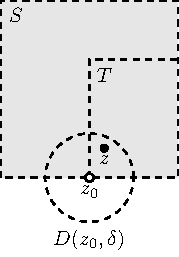
\includegraphics[scale=1]{ch1_subset1}
\caption{A subset $T$ of $S$ and a point $z_0$ that is a limit point of both $T$ and $S$.}
\end{SCfigure}
What can we say about $\rlim{z \to z_0}{z \in T} f(z)$?
\end{question}
\begin{answer}
Let $\epsilon >0$ be given, then we know that there exists $\delta >0$ such that
\[
z \in S,\ 0<|z-z_0|<\delta \ \Rightarrow |f(z)-\alpha| < \epsilon.
\]
Note that
\[
 z \in D'(z_0, \delta) \cap T \text{ implies } z \in D' (z_0,\delta) \cap S,
\]
or in other words,
\[
z \in T\ \text{ and } 0 < \abs{z -z_0} < \delta \Rightarrow z \in S \text{ and } 0 < \abs{z-z_0} < \delta.
\]

It follows that
\[
 \lim_{\substack{z \to z_0 \\ z \in S}} f(z) = \alpha \text{ implies }  \lim_{\substack{z \to z_0 \\ z \in T}} f(z) = \alpha
\]
\end{answer}
The second limit, where $f$ is restricted to the subset $T$ of $S$, is called a \emph{restricted limit}.   If a function has a limit at a point $z_0$ then all restricted limits of that function at $z_0$ must be the same.   In particular, 

\emph{If we have two subsets $T_1,T_2 \subseteq S$ such that 
\[
 \lim_{\substack{z \to z_0 \\ z \in T_1}} f(z) = \alpha_1 \text{ and } \lim_{\substack{z \to z_0 \\ z \in T_2}} f(z) = \alpha_2,
\]
with $\alpha_1 \neq \alpha_2$, then
\[
\lim_{\substack{z \to z_0 \\ z \in S}} f(z)
\]
does not exist.
}




Let $f$ be a complex function with domain $S$ and let $z_0$ be a limit point of $S$.  In what follows, we shall simply write $\displaystyle \lim_{z \to z_0} f(z)$ in place of \[
\lim_{\substack{z \to z_0 \\ z \in S}} f(z),
\]
and we shall reserve the second subscript for restricted limits.



\begin{example}
\label{e:rlim}
Consider the function 
\[
f: \C \backslash \set{0} \to \C, \quad f(z) = \frac{\conj{z}}{z}.
\]
Does 
$
\displaystyle \lim_{z \to 0} f(z)
$
exist?
\end{example}
\begin{note}
In future, we may simply write things like ``Let $f(z) = \dfrac{\conj{z}}{z}$'' without specifying the domain, since it is clear that this function $f$ is defined on $\C \backslash \set{0}$.
\end{note}
\begin{solution}
We shall look at two restricted limits of $f(z)$ as $z$ approaches $0$, namely the limits when $z$ is restricted to the subsets
\begin{itemize}
\item the nonzero real axis $\R \backslash \set{0}$, and
\item the nonzero imaginary axis $i \R \backslash \set{0}$ (Since every point on the imaginary axis is of the form $iy$ for some $y \in \R$, it makes sense to use the notation $i \R$ for this set.)
\end{itemize}
of the domain $\C \backslash \set{0}$.  Note that $0$ is a limit point of both $\R \backslash \set{0}$ and $i\R \backslash \set{0}$.

%\begin{center}
%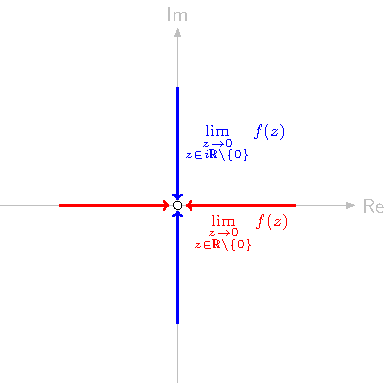
\includegraphics[scale=1]{origin_full}
%\end{center}

If $z \in \R \backslash \set{0}$, then $\conj{z} = z$ and so $f(z) = \frac{\conj{z}}{z} = \frac{z}{z} =1$ on $\R \backslash \set{0}$.  Hence
\[
\rlim{z \to 0}{z \in \R \backslash \set{0} } f(z)=1.
\]
For $z \in i \R \backslash \set{0}$, we have $\conj{z}=-z$, so that $f(z)=-1$ for all such $z$, giving
\[
\rlim{z \to 0}{z \in i\R \backslash \set{0} }=-1.
\]
Since  these limits are not equal, it follows that the (unrestricted) limit $\lim_{z \to 0} f(z)$ does not exist.
%\vspace*{12cm}
\end{solution}


\section{Continuity}

\begin{definition}
Let $S \subseteq \C$ and let $f:S \to \C$ be given.  For a point $z_0 \in S$, we say that $f$ is \emph{continuous at $z_0$} if $\lim_{z \to z_0 } f(z)=f(z_0)$. If $f$ is continuous at all points $z_0 \in S$ then we say that $f$ is \emph{continuous on $S$}.
\end{definition}
\begin{note}
Note that the definition of continuity at $z_0$ only makes sense when $z_0$ belongs to the domain of $f$.
\end{note}


\begin{example}
\label{e:cts}

The functions
\begin{enumerate}
\item[(i)] $f(z) = \Re (z)$,
\item[(ii)] $f(z) = \Im (z)$, and
\item[(iii)] $f(z) = \conj{z}$
\end{enumerate}
are all continuous on $\C$.
\end{example}

\begin{solution}
Fix $z_0=x_0+iy_0 \in \C$ and let $\epsilon>0$ be given.  Note that for any $z=x+iy \in \C$ we have the following inequalities:
\begin{align*}
\abs{ \Re (z) - \Re (z_0)} = \abs{\Re (z-z_0)} & = \sqrt{(x-x_0)^2} \\
&\leq \sqrt{(x-x_0)^2+(y-y_0)^2} = \abs{z-w} \\
\abs{ \Im (z) - \Im (z_0)} = \abs{\Im (z-z_0)} & = \sqrt{(y-y_0)^2} \\
&\leq \sqrt{(x-x_0)^2+(y-y_0)^2} = \abs{z-z_0} \\
\abs{\conj{z}-\conj{z_0}} = \abs{\conj{z-z_0}} & = \abs{z-z_0}.
\end{align*}
Thus in all three cases, setting $\delta=\epsilon$, we get
\[
0< \abs{z-z_0} < \delta \Longrightarrow \abs{f(z)-f(z_0)} < \epsilon.
\]
\end{solution}



\begin{proposition}
\label{t:continuity}
Let $S \subseteq \C$ and let $f,g:S \to \C$ be functions that are continuous on $S$.  Then
\begin{enumerate}
\item[(i)] The function $f+g,$ where $(f+g)(z)=f(z)+g(z)$, is continuous on $S$,
\item[(ii)] The function $fg$, where $(fg)(z):=f(z)g(z)$, is continuous on $S$,
\item[(iii)] For any $\alpha \in \C$, the function $\alpha f$, where $(\alpha f)(z)=\alpha \left( f(z) \right),$ is continuous on $S$,
\item[(iv)] If $T=\set{z \in S: g(z) \neq 0 }$ then the function $ f/g$, where $ \left( \dfrac{f}{g} \right) (z)= \dfrac{f(z)}{g(z)},$ is continuous on $T$.
\end{enumerate}
\end{proposition}
{\bf Proof:} Immediate from Proposition~\ref{p:alglimits}.

\begin{note}
If we have
\[
f(x+iy) = u(x,y) + i v(x,y),
\]
and $z_0 = x_0 + i y_0$ is a point in the domain of $f$, then
\[
\lim_{z \to z_0} f(z) = \lim_{(x,y) \to (x_0,y_0)} u(x,y)+ i \lim_{(x,y) \to (x_0,y_0)} v(x,y),
\]
provided these limits exist.  Hence
\[
f \text{ continuous at }z_0 \Leftrightarrow u \text{ and } v \text{ continuous at } (x_0,y_0).
\]
This is useful when the real and imaginary parts of $f$ are familiar functions that we know to be continuous.
\end{note}

\newpage



